\documentclass[11pt,a4paper]{article}
\usepackage[utf8]{inputenc}
\usepackage[vietnamese]{babel}
\usepackage{amsmath,amssymb}
\usepackage[version=4]{mhchem}
\usepackage{geometry}
\geometry{top=1.5cm,bottom=1.2cm,left=1.4cm,right=1.4cm,headheight=28pt,headsep=12pt,footskip=18pt}
\usepackage{graphicx}
\usepackage{xcolor}
\usepackage{tabularx}
\usepackage{array}
\usepackage{colortbl}
\usepackage{tikz}
\usepackage{fancyhdr}
\usepackage{enumitem}
\usepackage{multido}
\usepackage{tcolorbox}

\definecolor{hfRed}{HTML}{D32F2F}
\definecolor{hfGreen}{HTML}{8BC390}
\definecolor{mainGreen}{HTML}{2E7D32}
\definecolor{solBlue}{HTML}{1565C0}
\definecolor{tableGreen}{HTML}{E8F5E9}

\usepackage{ex_test}

\pagestyle{fancy}
\fancyhf{}
\renewcommand{\headrulewidth}{0.75pt}
\renewcommand{\headrule}{\hbox to\headwidth{\color{hfGreen}\leaders\hrule height \headrulewidth\hfill}}
\renewcommand{\footrulewidth}{0.75pt}
\renewcommand{\footrule}{\hbox to\headwidth{\color{hfGreen}\leaders\hrule height \footrulewidth\hfill}}

\fancyhead[L]{\small\itshape\color{hfRed}Tài liệu lưu hành nội bộ}
\fancyhead[R]{\small\color{hfRed}Thầy \textbf{TRẦN VĂN THẠNH} - 0777.470.803}

\fancyfoot[L]{\footnotesize\itshape\color{hfRed}CS1: 6/15 Nguyễn Hoàng, P. Kim Long, TP Huế \quad|\quad CS2: 24 Đặng Thái Thân, TP Huế}
\fancyfoot[R]{\small\textbf{\color{hfRed}Trang \thepage}}

\setlength{\parindent}{0pt}
\setlength{\parskip}{2pt}

\begin{document}

\begin{minipage}[t]{0.48\textwidth}
\textbf{SỞ GIÁO DỤC \& ĐÀO TẠO}\\
\textbf{TRƯỜNG THPT CAO THẮNG}\\
\textit{ĐỀ CHÍNH THỨC}\\
\textit{(Đề thi có 04 trang)}
\end{minipage}
\hfill
\begin{minipage}[t]{0.48\textwidth}
\raggedleft
\textbf{\color{hfRed}ĐỀ KIỂM TRA CUỐI KÌ 1}\\
\textbf{NĂM HỌC 2024 -- 2025}\\
\textbf{MÔN: HÓA HỌC 11}\\
\textit{Thời gian làm bài: 45 phút (không kể thời gian giao đề)}\\
\textbf{MÃ ĐỀ: 324}
\end{minipage}

\vspace{4pt}
\noindent
\textit{Họ và tên:} \dotfill \textit{Số báo danh:} \dotfill

\vspace{3pt}
\noindent
\textit{\footnotesize Cho biết nguyên tử khối: $\ce{H}=1;\ \ce{O}=16;\ \ce{C}=12;\ \ce{N}=14;\ \ce{Ca}=40;\ \ce{Fe}=56;\ \ce{S}=32;\ \ce{P}=31$.}

\vspace{3pt}
\hrule color{hfGreen} height 0.5pt

\vspace{4pt}
\noindent
{\color{mainGreen}\textbf{\Large A. TRẮC NGHIỆM KHÁCH QUAN (8,0 ĐIỂM)}}

\vspace{3pt}
\noindent
{\color{mainGreen}\textbf{\large PHẦN I. Câu trắc nghiệm nhiều phương án lựa chọn (3,5 điểm).}}\\
\textit{\small Thí sinh trả lời từ câu 1 đến câu 14. Mỗi câu hỏi thí sinh chỉ chọn một phương án.}
\vspace{2pt}

\begin{ex}
Ứng dụng nào sau đây không phải của sulfur dioxide?
\choice
{Sản xuất sulfuric acid}
{\True Sản xuất phân bón}
{Chống nấm mốc cho lương thực, thực phẩm}
{Tẩy trắng giấy, bột giấy}
\end{ex}
\begin{ex}
Phân tử ammonia có dạng hình học nào sau đây?
\choice
{\True Chóp tam giác}
{Tam giác đều}
{Chữ T}
{Chóp tứ giác}
\end{ex}
\begin{ex}
Công thức phân tử cho biết thông tin nào sau đây về phân tử hợp chất hữu cơ?
\choice
{Thành phần nguyên tố và tỉ lệ số lượng nguyên tử của mỗi nguyên tố}
{\True Thành phần nguyên tố và số lượng nguyên tử của mỗi nguyên tố}
{Số lượng nguyên tử mỗi nguyên tố và trật tự liên kết giữa các nguyên tử}
{Tỉ lệ số lượng nguyên tử của mỗi nguyên tố và trật tự liên kết giữa các nguyên tử}
\end{ex}
\begin{ex}
Tại nhiệt độ không đổi, ở trạng thái cân bằng,
\choice
{\True nồng độ của các chất trong phản ứng không thay đổi}
{phản ứng hoá học không xảy ra}
{tốc độ phản ứng hoá học xảy ra chậm dần}
{nồng độ của các chất trong phản ứng vẫn liên tục thay đổi}
\end{ex}
\begin{ex}
Nitric acid là một acid có tính oxi hóa mạnh. Do đó, nitric acid oxi hóa được hầu hết kim loại, trừ vàng (Au), platinum (Pt),... Tuy nhiên, Au và Pt có thể bị hòa tan trong nước cường toan, là hỗn hợp nitric acid đặc và hydrochloric acid đặc có tỉ lệ thể tích là
\choice
{2:3}
{3:1}
{1:1}
{\True 1:3}
\end{ex}
\begin{ex}
Tính chất nào sau đây không phải tính chất vật lí của sulfur?
\choice
{Thể rắn ở điều kiện thường}
{\True Không tan trong benzene}
{Màu vàng ở điều kiện thường}
{Không tan trong nước}
\end{ex}
\begin{ex}
``Đất phèn'' là một khái niệm dân gian để chỉ loại đất chứa nhiều ion sulfate, có $\text{pH} < 7$. Môi trường của đất phèn là
\choice
{môi trường trung hòa}
{môi trường base}
{môi trường trung tính}
{\True môi trường acid}
\end{ex}
\begin{ex}
Chất nào sau đây có chứa nhóm chức alcohol?
\choice
{$\ce{CH3CHO}$}
{$\ce{CH3COCH3}$}
{$\ce{CH3NH2}$}
{\True $\ce{C2H5OH}$}
\end{ex}
\begin{ex}
Trong tự nhiên, nguyên tố nitrogen tồn tại chủ yếu ở dạng đồng vị nào sau đây?
\choice
{$^{15}\ce{N}$}
{\True $^{14}\ce{N}$}
{$^{13}\ce{N}$}
{$^{12}\ce{N}$}
\end{ex}
\begin{ex}
Cặp chất nào sau đây là đồng đẳng của nhau?
\choice
{\True $\ce{CH3CH2CH3}$ và $\ce{CH3CH3}$}
{$\ce{CH3CH2CH2CH3}$ và $\ce{(CH3)2CHCH3}$}
{$\ce{CH3CH=CH2}$ và $\ce{CH3CH2CH2CH3}$}
{$\ce{CH2=CH-CH=CH2}$ và $\ce{CH3C#CH}$}
\end{ex}
\begin{ex}
Cho iron (III) oxide tác dụng với nitric acid thì sản phẩm thu được là:
\choice
{\True $\ce{Fe(NO3)3}$ và $\ce{H2O}$}
{$\ce{Fe(NO3)3}$, $\ce{NO2}$ và $\ce{H2O}$}
{$\ce{Fe(NO3)3}$, $\ce{N2}$ và $\ce{H2O}$}
{$\ce{Fe(NO3)3}$, $\ce{NO}$ và $\ce{H2O}$}
\end{ex}
\begin{ex}
Trong các hợp chất sau, chất nào là dẫn xuất của hydrocarbon?
\choice
{$\ce{C7H8}$}
{$\ce{C4H4}$}
{\True $\ce{CH3NH2}$}
{$\ce{C2H2}$}
\end{ex}
\begin{ex}
Dãy gồm các chất đều tác dụng với sulfur (trong điều kiện thích hợp của phản ứng) là:
\choice
{Au, Pt, Ag}
{Ag, $\ce{O2}$, $\ce{Cl2}$}
{\True Fe, Hg, $\ce{O2}$}
{Fe, Hg, C}
\end{ex}
\begin{ex}
Tín hiệu phổ hồng ngoại của một số nhóm chức cơ bản được cho ở Bảng (a) và Phổ hồng ngoại (IR) của hợp chất hữu cơ X được cho ở Hình (b).
\begin{center}
\renewcommand{\arraystretch}{1.1}
\begin{tabular}{|l|c|}
\hline
\rowcolor{tableGreen}
\textbf{Hợp chất} & \textbf{Số sóng ($\text{cm}^{-1}$)} \\
\hline
Alcohol & $3600 - 3300\ (\ce{O-H})$ \\
\hline
Amine & $3500 - 3300\ (\ce{N-H})$ \\
\hline
Aldehyde & $2900 - 2700\ (\ce{C-H});\ 1740 - 1720\ (\ce{C=O})$ \\
\hline
Ketone & $1725 - 1700\ (\ce{C=O})$ \\
\hline
Carboxylic acid & $3300 - 2500\ (\ce{O-H});\ 1725 - 1700\ (\ce{C=O})$ \\
\hline
Ester & $1750 - 1735\ (\ce{C=O});\ 1300 - 1000\ (\ce{C-O})$ \\
\hline
\end{tabular}
\end{center}
\begin{center}
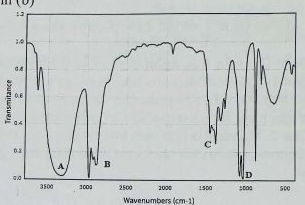
\includegraphics[width=8.0cm]{San_Pham/images_de324/hinh_b_ir_crop.png}
\end{center}
Phát biểu nào sau đây là đúng?
\choice
{Peak A và peak D cho thấy X là một carboxylic acid}
{\True Peak A là tín hiệu của nhóm OH}
{Peak C là tín hiệu của nhóm chức $\ce{C=O}$}
{Peak B và peak D cho thấy X là một aldehyde}
\end{ex}
\vspace{4pt}
\noindent
{\color{mainGreen}\textbf{\large PHẦN II: Câu trắc nghiệm đúng sai (3,0 điểm).}}\\
\textit{\small Thí sinh trả lời từ câu 1 đến câu 3. Trong mỗi ý a), b), c), d) ở mỗi câu, thí sinh chọn đúng hoặc sai.}
\vspace{2pt}

\begin{ex}
Một hợp chất hữu cơ X được xác định có công thức đơn giản nhất là $\ce{CH2O}$. Bằng phổ khối lượng MS, người ta xác định được phân tử khối của X là 60.
\choiceTF
{\True X là dẫn xuất hydrocarbon}
{\True Công thức phân tử của X là $\ce{C2H4O2}$}
{Thành phần phần trăm theo khối lượng của nguyên tố carbon trong X là $44\%$}
{Nếu X chỉ chứa một nhóm chức thì X có 3 đồng phân cấu tạo}
\end{ex}
\begin{ex}
Sulfuric acid là một trong những hoá chất quan trọng nhất được sử dụng trong công nghiệp; được sản xuất hàng trăm triệu tấn mỗi năm, chiếm nhiều nhất trong ngành công nghiệp hoá chất. Phương pháp sản xuất sulfuric acid phổ biến nhất là phương pháp tiếp xúc, theo đó acid có thể được điều chế qua các giai đoạn sau:
\begin{align*}
(1) &\quad 4\ce{FeS2} + 11\ce{O2} \xrightarrow{t^\circ} 2\ce{Fe2O3} + 8\ce{SO2} \\
(2) &\quad 2\ce{SO2}(g) + \ce{O2}(g) \xrightleftharpoons[\text{V}_2\text{O}_5]{450^\circ\text{C}} 2\ce{SO3}(g);\quad \Delta_r H^\circ_{298} = -196\text{ kJ} \\
(3) &\quad \ce{H2SO4} + n\ce{SO3} \longrightarrow \ce{H2SO4.nSO3} \\
(4) &\quad \ce{H2SO4.nSO3} + n\ce{H2O} \longrightarrow (n+1)\ce{H2SO4}
\end{align*}
\choiceTF
{Có ba phản ứng oxi hóa – khử đã xảy ra trong các giai đoạn sản xuất sulfuric acid trên}
{Để làm tăng hiệu suất tổng hợp $\ce{SO3}$ ở phản ứng (2) cần tăng nhiệt độ của phản ứng trên $450^\circ\text{C}$}
{Ở phản ứng (3), có thể dùng nước hấp thụ trực tiếp $\ce{SO3}$ để tạo thành $\ce{H2SO4}$ với nồng độ cao}
{\True Để sản xuất được 1 tấn dung dịch $\ce{H2SO4}$ $98\%$ cần 1 tấn quặng pyrite chứa $75\%\ \ce{FeS2}$. Biết hiệu suất của cả quá trình điều chế đạt $80\%$ và các tạp chất trong quặng không chứa sulfur}
\end{ex}
\begin{ex}
Thí nghiệm tách $\beta$-carotene từ nước ép cà rốt được thực hiện như sau:\\
- Bước 1: Cho khoảng $20\text{ mL}$ nước ép cà rốt vào phễu chiết. Thêm tiếp khoảng $20\text{ mL}$ hexane, lắc đều khoảng 2 phút.\\
- Bước 2: Để yên phễu chiết trên giá thí nghiệm khoảng 5 phút để chất lỏng tách thành hai lớp.\\
- Bước 3: Mở khoá phễu chiết cho phần nước chảy xuống, còn lại phần dung dịch $\beta$-carotene hoà tan trong hexane.
\choiceTF
{\True Phễu chiết tách thành hai lớp, lớp bên trên là $\beta$-carotene hoà tan trong hexane, lớp dưới là nước}
{\True Thí nghiệm tách $\beta$-carotene từ nước ép cà rốt dựa theo nguyên tắc chiết lỏng – lỏng}
{\True Dùng dung môi là hexane có khả năng hoà tan $\beta$-carotene nhưng không tan trong nước và có nhiệt độ sôi thấp để chiết}
{\True Sau bước 3, để thu được $\beta$-carotene người ta đun nóng để loại bỏ dung môi hexane}
\end{ex}
\vspace{4pt}
\noindent
{\color{mainGreen}\textbf{\large PHẦN III: Câu trắc nghiệm yêu cầu trả lời ngắn (1,5 điểm).}}\\
\textit{\small Thí sinh trả lời từ câu 1 đến câu 6. Thí sinh điền kết quả vào ô trả lời tương ứng.}
\vspace{2pt}

\begin{ex}
Cho cân bằng hóa học: $\ce{N2O4}(g) \rightleftharpoons 2\ce{NO2}(g)$. Ban đầu có $0,02\text{ mol}\ \ce{N2O4}$ trong bình kín có thể tích $500\text{ mL}$. Khi phản ứng đạt trạng thái cân bằng, nồng độ của $\ce{N2O4}$ là $0,0055\text{ M}$. Tính hằng số cân bằng $K_c$. \textit{(Kết quả làm tròn đến hàng phần trăm)}.
\hfill \textbf{Trả lời:} \dotfill
\end{ex}
\begin{ex}
Menthol là hợp chất hữu cơ được tìm thấy trong cây bạc hà. Nó được sử dụng làm hương liệu trong nhiều chất như: kem đánh răng, kẹo cao su và xi-rô ho,... menthol có công thức cấu tạo là:
\begin{center}
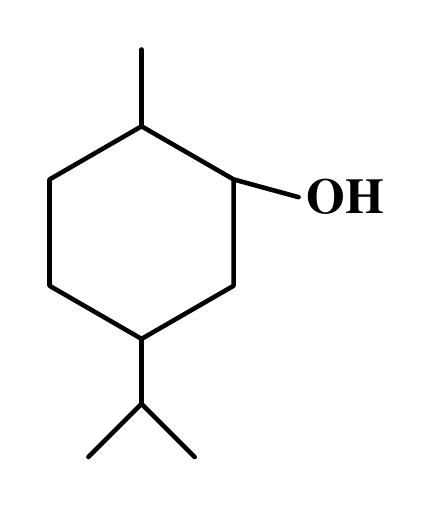
\includegraphics[width=3.5cm]{San_Pham/images_de324/menthol.png}
\end{center}
Tổng số nguyên tử có trong phân tử menthol là bao nhiêu?
\hfill \textbf{Trả lời:} \dotfill
\end{ex}
\begin{ex}
Cho các chất khí: $\ce{NO, NO2, SO2, N2O}$ và $\ce{N2}$. Có bao nhiêu chất khí là nguyên nhân góp phần gây ra hiện tượng mưa acid?
\hfill \textbf{Trả lời:} \dotfill
\end{ex}
\begin{ex}
Cho dãy các chất sau: $\ce{HClO4, HClO, Mg(OH)2, HNO3, KH2PO4, Ca(OH)2, NaCl, CuSO4, CH3COOH}$. Có bao nhiêu chất trong dãy thuộc loại chất điện li mạnh?
\hfill \textbf{Trả lời:} \dotfill
\end{ex}
\begin{ex}
Cho các chất có công thức cấu tạo sau:
\begin{center}
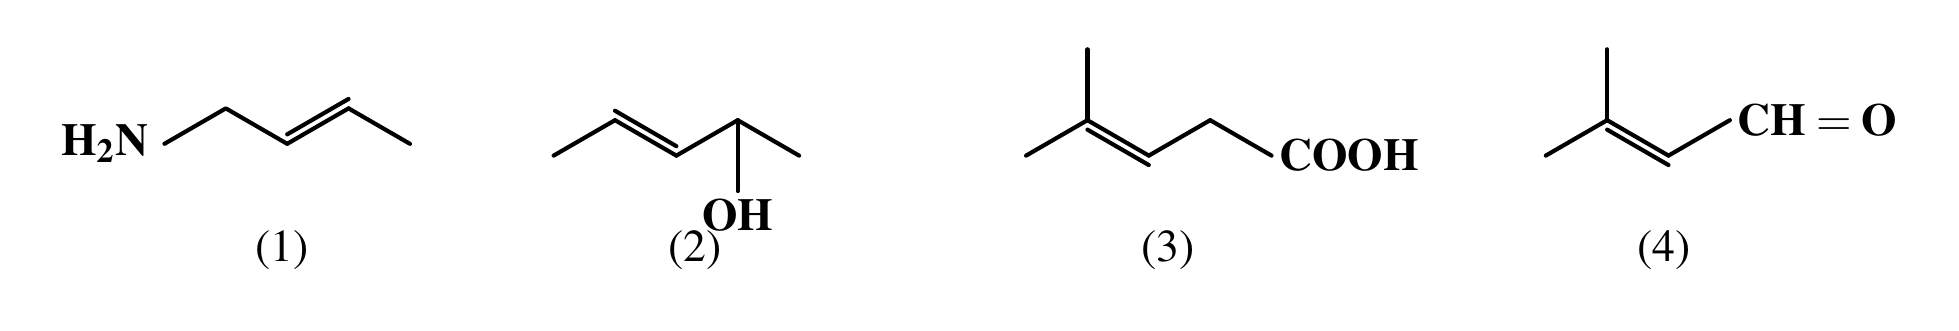
\includegraphics[width=13.0cm]{San_Pham/images_de324/cau5_4chat.png}
\end{center}
Có bao nhiêu chất trong các chất trên có tín hiệu trên phổ hồng ngoại ở khoảng tần số $1750 - 1680\text{ cm}^{-1}$? Xem bảng tín hiệu phổ hồng ngoại của một số nhóm chức cơ bản ở phần I-Trắc nghiệm nhiều phương án lựa chọn.
\hfill \textbf{Trả lời:} \dotfill
\end{ex}
\begin{ex}
Cho phương trình hóa học của các phản ứng sau:
\begin{align*}
(1) &\quad 8\ce{NH3} + 3\ce{Cl2} \longrightarrow 6\ce{NH4Cl} + \ce{N2} \\
(2) &\quad 4\ce{NH3} + 5\ce{O2} \xrightarrow{t^\circ, \text{Pt}} 4\ce{NO} + 6\ce{H2O} \\
(3) &\quad 2\ce{NH3} + \ce{H2SO4} \longrightarrow (\ce{NH4})_2\ce{SO4} \\
(4) &\quad 2\ce{NH3} + 3\ce{CuO} \xrightarrow{t^\circ} \ce{N2} + 3\ce{Cu} + 3\ce{H2O} \\
(5) &\quad \ce{MgCl2} + 2\ce{NH3} + 2\ce{H2O} \longrightarrow \ce{Mg(OH)2}\downarrow + 2\ce{NH4Cl}
\end{align*}
Có bao nhiêu phản ứng hóa học trong đó ammonia đóng vai trò là chất khử?
\hfill \textbf{Trả lời:} \dotfill
\end{ex}
\vspace{4pt}
\noindent
{\color{mainGreen}\textbf{\Large B. PHẦN TỰ LUẬN (2,0 ĐIỂM)}}

\vspace{3pt}

\noindent
\textbf{Câu 1. (1,0 điểm)} Tại một công ty superphosphate và hóa chất, superphosphate kép được sản xuất từ quặng phosphorite theo hai giai đoạn sau:
\begin{align*}
\ce{Ca3(PO4)2 + 3H2SO4} &\longrightarrow \ce{2H3PO4 + 3CaSO4} \\
\ce{Ca3(PO4)2 + 4H3PO4} &\longrightarrow \ce{3Ca(H2PO4)2}
\end{align*}
Trung bình mỗi ngày, công ty sản xuất được $1872\text{ tấn}\ \ce{Ca(H2PO4)2}$, giả thiết hiệu suất của mỗi giai đoạn đạt $100\%$. Tính thể tích dung dịch $\ce{H2SO4}\ 70\%\ (D = 1,6\text{ tấn/m}^3)$ mà công ty đã dùng trong một ngày.

\vspace{2pt}
\multido{\i=1+1}{8}{\noindent\dotfill\\}

\vspace{4pt}
\noindent
\textbf{Câu 2. (1,0 điểm)} Hợp chất hữu cơ X (mạch hở) được dùng làm dung môi trong quá trình tổng hợp dược phẩm. Kết quả phân tích nguyên tố của X như sau: $64,864\%\ce{C}$; $13,514\%\ce{H}$ về khối lượng và còn lại là oxygen. Phân tử khối của X được xác định thông qua kết quả phổ khối lượng với peak ion phân tử có giá trị $m/z$ lớn nhất bằng 74.\\
a. Hãy xác định công thức phân tử chất hữu cơ X.\\
b. Trong phổ hồng ngoại (IR), chất X có số sóng hấp thụ đặc trưng trong khoảng $3500 - 3200\text{ cm}^{-1}$. Hãy viết các đồng phân cấu tạo của X thỏa mãn điều kiện trên. Xem bảng tín hiệu phổ hồng ngoại của một số nhóm chức cơ bản ở phần I-Trắc nghiệm nhiều phương án lựa chọn.

\vspace{2pt}
\multido{\i=1+1}{8}{\noindent\dotfill\\}

\vspace{8pt}
\begin{center}
\textbf{---------- HẾT ----------}
\end{center}

\end{document}
